\chapter{Evaluation of multiple access strategies with power control error 
and variable packet length in M2M}

% **************************** Define Graphics Path **************************
\ifpdf
    \graphicspath{{Chapter3/Figs/Raster/}{Chapter3/Figs/PDF/}{Chapter3/Figs/}}
\else
    \graphicspath{{Chapter3/Figs/Vector/}{Chapter3/Figs/}}
\fi

Based on WCNC2016
Machine-to-machine (M2M) communication is expected to enable billions of devices to be connected by the cellular networks in the near future. The large number of devices involved in M2M will create a huge market potential but at the same time pose some challenges for 3GPP cellular networks. The challenges include massive access management, QoS provisioning, energy/power efficiency, etc. Nowadays, energy-related issues are deemed as the key problems in cellular M2M communications. In this paper, we extend the research framework of \cite{Dhi13} by taking into account some important issues that were not yet addressed, mainly the existence of machines with different packet lengths and the effect of imperfect power control. With the proposed system model, we evaluate the power efficiency, energy efficiency and system capacity for uncoordinated CDMA and coordinated FDMA. Through numerical results, we conclude that coordinated FDMA is more resistant to various packet lengths of M2M devices packets in terms of power efficiency and is not influenced by imperfect power control. Thus coordinated multiple strategies, especially FDMA, are more suitable for the future M2M-included cellular networks and deserve further optimization works. With respect to uncoordinated CDMA, although its performance is affected by BS load intensity and power control, it is still a considerable choice due to its simplicity and no signaling overhead, when the BS load intensity is not high and the power control policy is suitable. 

The remainder of this paper is organized as follows: an introduction about our system model is given in Sec.~\ref{sec:system-model}, presenting some basic hypothesis, multiple access methods to be compared and selected performance metric.  
Sec.~\ref{sec:uncoordinated-strategy} is devoted to analyze the performance of uncoordinated strategy, mainly for CDMA. 
Sec.~\ref{sec:coord-strategy} discusses the performance of coordinated strategies. 
Sec.~\ref{sec:numerical-res} shows the numerical result by using the conclusions from the previous two sections.
Finally, Sec.~\ref{sec:conclusion} concludes the paper by summarizing the main findings of the paper.

\section{Introduction}
Machine-to-machine (M2M) communication, also called Machine type communication (MTC) in 3GPP's terminology, refers to an emerging technology which enables machine devices to be connected to a wide-area cellular network. This promising technology is expected to facilitate the creation of new applications and business models. In terms of carrier networks, due to the ubiquitous coverage, mature subscription management system, the 3GPP cellular networks are the best candidates for handling M2M traffic. As an example, it is estimated that over $2$ billion M2M devices will be connected to cellular networks in $2020$ \cite{Eri11}.

The integration of M2M into current cellular networks poses many challenges, since M2M traffic exhibits completely different characteristics from human-to-human (H2H) such as: a large number of short sessions, a number of battery operated devices, difficulty of replacing or recharging batteries for devices, and so on. In the past, mobile cellular networks were designed with objectives of maximizing spectral efficiency and minimizing latency. Nowadays, in the evolution from 4G to 5G, the differences between these two communication paradigms (H2H and M2M) should be considered and some design principles shifts are required.   

In the literature, lots of research efforts are made to mitigate the challenges imposed by the M2M traffic. The issue of Radio Access Network (RAN) overload control is identified as the first improvement area by 3GPP \cite{3GPP/TS/37868V11}, which leads to plenty of proposals for reducing random access collision and latency. Progressively, energy related issues (i.e., energy efficiency, power efficiency, etc.) are deemed as the key problems that determines if M2M communication is accepted as a promising communication technology \cite{lu11GRS}. To this end, diverse aspects are exploited by research community. Some researchers apply cooperative design such as clustering method \cite{YuanHo12}\cite{azari14}. Discontinuous reception (DRX) and Idle state in LTE/LTE-A are further optimized in \cite{Gupta2013}. Random access procedure is simplified by leveraging the transmission of small payload in \cite{ChenY10machine}. New radio resource allocation algorithms are proposed to achieve energy efficiency/saving \cite{AijazTNCA14}. Some researchers also consider to avoid random access procedure by leveraging the periodicity feature of M2M \cite{qipeng2015an}.
However, there are few works about the performance evaluation in terms of energy efficiency or power efficiency for frequently used multiple access strategies (e.g., CDMA/FDMA/TDMA). To our best knowledge, Dhillion et al.~\cite{Dhi13} made the first trial and proposed a system model to compare the multiple access mechanisms such as CDMA/FDMA/TDMA with metric of power efficiency and energy efficiency, but their work has not covered some factors important in real networks. For instance, the packet length is constant and the power control is ignored in \cite{Dhi13}. In this paper, we consider the aforementioned ignored factors and extend the system model in order to reevaluate the performance between CDMA and FDMA, and verify whether their obtained design guides are still valid in the extended system model.
\section{System model}
\label{sec:system-model}
% 描述其数学模型,同时指出不足(改进方向)
% 无比纠结中:原论文中,诸如不考虑重传,不考虑overhead signaling,etc啥的。。。要不要提呢?提了是抄袭 不提是model中的漏洞
\subsection{Description and hypothesis}
\qs{xxx}
The system model is mainly extended from the one proposed by \cite{Dhi13}  and is described in the following lines: a single cell consisting of an access point is situated at the origin of a circle area. All devices are uniformly distributed around the origin in an annular region with inner and outer radii $r_{i}$ and $r_{0}$. The probability density function of distance between a device and cell origin $r$ is the following \cite{5341148}:
\begin{align}
	f_R\left( r\right) = \frac{2r}{r_0^2-r_i^2},  r_i \leq r \leq r_0
\end{align}
The non-zero inner radius $r_i$ is assumed to avoid singularity in the path loss model. The multi-cell case is currently out of the scope of our work and thus the out-of-cell interference is not taken into account. The proposed system model is assumed to be a slotted system with $\tau_s$ time slot duration. The multiplexing access is performed on a time-frequency resource slice with duration $\tau_s$ and bandwidth $W$. The arrival process of packets in the uplink is modeled as a Poisson point process with mean $\lambda$ arrivals per second. Therefore, the number of packet transmission request $N_a$ in duration $\tau_s$ respects to Poisson distribution demoted by $N_{a} \sim Pois(\lambda \tau_{s})$. The M2M devices present in the cell are managed by diverse applications and each application has a different packet length. Thus the packet length $l$ varies from $\left[L_{0}, L_{1}\right]$. We further assume that the devices perform uplink power control, but the power control is imperfect.
\subsection{Multiple access strategies}
Two types of multiple access strategies are considered in the system model: \begin{inparaenum}[i)]
	\item uncoordinated: the devices transmit data and control information using slotted random access without establishing dedicated radio bearer;
	\item coordinated: the devices transmit data in a separate scheduled radio resource after a random access contention.
\end{inparaenum}
The most frequent uncoordinated strategies are CDMA and FDMA. Compared with CDMA, the system capacity of uncoordinated FDMA is rather limited \cite{Dhi13}, which is by nature unsuitable for handling M2M traffic. Thus, we just consider CDMA in uncoordinated strategies. For the same reason, in coordinated case, just coordinated FDMA is considered.   
\subsection{Performance metrics}
% 这里可以继续 论证下 为什么我就可以选择这几个 标准呢
In our system model, the power efficiency is defined as the average transmit power $\overline{P_t}$ for all involved M2M devices. The energy efficiency is measured by the average energy per bit $\overline{E_b}$. The average energy per bit $\overline{E_b}$ is the product of time (to transmit the packet) and average transmit power $\overline{P_t}$.  
Given that M2M applications usually consist of large number of devices, maximum supported base station load intensity $\lambda_{max}$ is used to evaluate the system capacity.
\subsection{Basic mathematical model for uplink}
%完全来自Dhillion的paper
The received power $P_r$ at the base station from a device located at distance $r$, assuming transmit power $P_t$, path loss exponent $\gamma$, small-scale fading gain $h$, large-scale shadowing gain $\chi$ and direct based antenna gain $G$ is:
\begin{align}
& P_r = P_t \chi h G r^{-\gamma} 
\end{align}
To facilitate the writing, two SNR values are defined, reference SNR $\mu_0$ and bandwidth-aware SNR $\mu$, as following:
\begin{align}
& \mu_0 = \frac{P_{max}Gr_0^{-\gamma}}{N_0W} \\
& \mu =  \mu_0\frac{W}{W_N} \label{eq:actual-reference-snr}
\end{align}
The reference SNR refers to the received SNR at the base station for a device at the cell edge (with distance $r_0$ to the the cell origin) transmitting at maximum power $P_{max}$ over total bandwidth $W$ when fading and shadowing effects are averaged out. The bandwidth-aware SNR is similar to the reference SNR except that the former is calculated over the actually occupied bandwidth $W_N$. The bandwidth-aware SNR is useful when analysing multiplex access strategies where frequency is divided into sub-channel such as FDMA. The received SNR $\mu_r$ at the base station for a device with distance $r$ to the center can be simply expressed as:
\begin{align}
& \mu_r = \frac{P_t}{P_{max}} \mu \chi h \left( \frac{r}{r_0} \right) ^{-\gamma} \label{eq:SNR-measured-by-reference-SNR}
\end{align}
To further simplify (\ref{eq:SNR-measured-by-reference-SNR}), the term $\chi h \left( \frac{r}{r_0} \right) ^{-\gamma}$ is defined as the relative channel gain \footnote{We prefer to denote \textbf{\textit{relatively channel gain}} instead of \textbf{\textit{channel gain}} as in \cite{Dhi13}.} denoted by $g$. 
%\footnote{The term channel gain in initial paper is misleading. It can be regarded as a normalized channel gain}. 
Then the received $\mu_r$ is simplified as:
\begin{align}
\mu_r = \frac{P_t}{P_{max}} \mu g \label{eq:received-snr}
\end{align}
For all analysis in this paper, an information symbol of payload $l$ bits will be transmitted over bandwidth $W_N \leq W $ for time $\tau \leq \tau_s$. According to Shannon's capacity formula, there exist two basic preliminaries for uncoordinated and coordinated strategies in terms of minimum transmission slot $\tau_{min}$ and minimum bandwidth $W_{min}$:
\begin{align}
& \tau_{min} = \frac{l}{W_{N}\log_{2}\left( 1+\mu_{N}g\right) } \label{constraint-time}\\
& \frac{l}{\tau W_{min}} = \log_{2} \left( 1+\mu\left( \frac{W}{W_{min}}\right) g\right)   \label{constraint-freq}
\end{align}
\section{Uncoordinated strategies}
\label{sec:uncoordinated-strategy}
For uncoordinated CDMA, the only information that the base station knows about the number of transmission is the estimation of mean load $\lambda\tau_s$ of Poisson distribution (estimated from the arrival history). The system with CDMA as multiple access mechanism is designed to serve $(1-\epsilon)$ percentile of the arrivals. The maximum supported users in each slot is denoted by $\overline{N}$ which satisfies $\mathbb{P}\left[N_a > \overline{N}\right] \leq \epsilon$. For this design, there exist three types of failure events which dictate the maximum load at base station:
\begin{inparaenum}[i)]
	\item $N_a > \overline{N}$, the actual arrival transmission request is more than the designed maximum supported users;
	\item resource selection collision, more than one user choose the same system resource, such as random access code in CDMA or sub-channel in FDMA;
	\item $P_t > P_{max}$, the required transmit power is greater than theoretical maximum transmit power. 
\end{inparaenum}
The conclusions obtained for uncoordinated CDMA in \cite{Dhi13} are resumed in Tab.~\ref{tab:uncoordinated-resume} and used as benchmark.
%\begin{table}[h]
%	\centering
%	\caption{Uncoordinated strategies performance resume}
%	\label{tab:uncoordinated-resume}
%	\begin{tabular}{@{}lcc@{}}
%		\toprule
%		& CDMA                                                                            & FDMA                                                                          \\ \midrule
%		Transmit \\ power      & $P_t=\frac{P_{max}}{\mu g \left( N_c\mu_t^{-1} - \overline{N}+1\right)}$        & $P_t=\frac{2^{\frac{LN_f}{W\tau_s}}-1}{\mu g N_f}P_{max}$                     \\ \midrule
%		Energy \\per bit      & $E_b=\frac{\tau_sP_{max}}{L\mu g \left( N_c\mu_t^{-1} - \overline{N}+1\right)}$ & $E_b=\frac{\tau_s\left(2^{\frac{LN_f}{W\tau_s}}-1\right)P_{max}}{L\mu g N_f}$ \\ \midrule
%		Failure \\probability & \multicolumn{2}{c}{$P_f \leq \epsilon + (1-\epsilon)\{\delta+(1-\delta)P_c\}$}                                                                                  \\ \midrule
%		Maximum \\load        & \multicolumn{2}{c}{$\lambda_{max} = max\{\lambda: \mathbb{P}\left[P_t(\lambda) > P_{max}\right] \leq \delta, P_f \leq p\}$}                                    \\ \bottomrule
%	\end{tabular}
%\end{table}
\begin{table}[h]
	\centering
	\caption{Uncoordinated strategies performance resume}
	\label{tab:uncoordinated-resume}
	\begin{tabular}{@{}lcc@{}}
		\toprule
		& CDMA                                                                                                                                        \\ \midrule
		Transmit  power      & $P_t=\frac{P_{max}}{\mu g \left( N_c\mu_t^{-1} - \overline{N}+1\right)}$                         \\ \midrule
		Energy per bit      & $E_b=\frac{\tau_sP_{max}}{l\mu g \left( N_c\mu_t^{-1} - \overline{N}+1\right)}$ \\ \midrule
		Failure probability & \multicolumn{2}{c}{$P_f \leq \epsilon + (1-\epsilon)\{\delta+(1-\delta)P_c\}$}                                                                                  \\ \midrule
		Maximum load        & \multicolumn{2}{c}{$\lambda_{max} = max\{\lambda: \mathbb{P}\left[P_t(\lambda) > P_{max}\right] \leq \delta, P_f \leq p\}$}                                    \\ \bottomrule
	\end{tabular}
\end{table}
In CDMA random access, each device is assumed to randomly select a code of length $N_{c}$ from the set of $2^{N_{c}}-1$ possible binary sequences, where $N_c$ is a design parameter. The CDMA waveform is transmitted over the total bandwidth $W$. The effective bandwidth of the information symbols is assumed as $W/N_{c}$. Devices are assumed to perform uplink power control such that the target SINR at the base station is $\mu_{t}$. We separately evaluate the impact of various packet length and imperfection of power control. Note that when analyzing the impact of various packet length, the power control is regarded as perfect and vice versa.

%the authors just give transmit power required for each device, but they do not show how to estimate the average transmit power of each strategy (CDMA, FDMA,etc.).  Here, I think the authors take the average of transmit power of all devices.

%From formula (\ref{eq:CDMA-transmit-power}) and $g=\chi h \left( \frac{r}{r_0}\right)^{-\gamma} $, we regard channel gain $r$ is random variable whose PDF is $f_R\left( r\right) = \frac{2r}{r_0^2-r_i^2}$, where $r \in \left[ r_i, r_0\right] $ \cite{5341148} and transmit power $p_t$ is function of random variable $r$, namely $p_t=h(r)$. Hence $p_t$ is also a random variable and average transmit power is the expectation of $p_t$. 
%\begin{align}
%\mathbb{E}\left[ p_t\right]=\mathbb{E}\left[ h(r)\right] &=\int_{-\infty}^{\infty} h\left( r\right) f_R \left( r\right) dr \nonumber\\
%&= \int_{r_i}^{r_0} \frac{P_{max}}{[\mu g (N_{c}\mu_{t}^{-1}-(\bar{N}-1))]} \cdot \frac{2r}{r_0^2-r_i^2} dr \nonumber\\
%\intertext{Since the fading and shadowing is averaged out}
%\mathbb{E}\left[ h(r)\right] &= \int_{r_i}^{r_0} \frac{P_{max}}{[\mu  \left( \frac{r}{r_0}\right)^{-\gamma} (N_{c}\mu_{t}^{-1}-(\bar{N}-1))]} \cdot \frac{2r}{r_0^2-r_i^2} dr \nonumber\\
%&= \int_{r_i}^{r_0} \frac{P_{max}}{[\mu  (N_{c}\mu_{t}^{-1}-(\bar{N}-1))]} \cdot \frac{2r}{r_0^2-r_i^2} \cdot \left( \frac{r}{r_0}\right)^{\gamma} dr \nonumber\\
%&= \int_{r_i}^{r_0} \frac{P_{max}}{[\mu  (N_{c}\mu_{t}^{-1}-(\bar{N}-1))]} \cdot \frac{2r_0^{-\gamma}}{r_0^2-r_i^2} \cdot r^{\gamma+1} dr \nonumber\\
%&= \frac{P_{max}}{[\mu (N_{c}\mu_{t}^{-1}-(\bar{N}-1))]} \cdot \frac{2r_0^{-\gamma}}{r_0^2-r_i^2}\cdot \frac{1}{\gamma+2}\cdot r^{\gamma+2} \mid^{r_0}_{r_i} \nonumber\\
%&= \frac{P_{max}}{[\mu (N_{c}\mu_{t}^{-1}-(\bar{N}-1))]} \cdot \frac{2r_0^{-\gamma}}{r_0^2-r_i^2}\cdot \frac{ r_0^{\gamma+2}-r_i^{\gamma+2}}{\gamma+2}
%\end{align}
\subsection{Impact of various packet length}
In a practical system, it is possible that the packet length sent by each device is not the same for all devices. In this section, we study the impact on performance metric such as average transmit power caused by variable packet length $l$ with system model proposed in Sec.~\ref{sec:system-model}. The power efficiency is measured by the average transmit power for all served devices in the coverage area of the cell. In case of CDMA, the devices are assumed to perform uplink power control such that the target SINR received at the base station is $\mu_t$. Assuming that $l$ bits are transmitted in each transaction (duration $\tau_s$), the effective bandwidth of the information symbols is denoted as $W/N_c$, therefore target SINR $\mu_t$ is defined as:
\begin{align}
\frac{l}{\tau_s} &= \frac{W}{N_c} \cdot \log_2 \left( 1+ \mu_t\right)  \nonumber \\
\mu_t &= 2^{\frac{lN_c}{W\tau_s}}-1 \label{eq:mut-lower-bound}
\end{align}
According to (\ref{eq:mut-lower-bound}) and transmit power of CDMA case given in Tab.~\ref{tab:uncoordinated-resume}, the interval of $\mu_t$ can be deduced as: 
\begin{align}
2^{\frac{lN_c}{W\tau_s}}-1 \leq \mu_t &< \frac{N_c}{\overline{N}-1} \label{eq:mut-upper-bound}
\end{align}
where CDMA code length $N_c$ is actually a function of BS load intensity $\lambda$. We now redefine target SNR as following by considering packet length as a variable $l$:
\begin{align}
\mu_t = 2^{\frac{l N_c}{W\tau_s}}-1
\end{align} 
With the inequality (\ref{eq:mut-upper-bound}), we determine the lower bound and upper bound of packet length $l$:
\begin{align}
L_{0} \leq l <L_{1} = \frac{W\tau_s}{N_c} {\log_2}^{\left( \frac{N_c +\overline{N} -1}{\overline{N}-1}\right) } \label{ieq:packet-length-interval}
\end{align} 
where $L_{1}$ refers to the maximal packet length given a BS load intensity and is the function of the latter. From maximum load given in Tab.~\ref{tab:uncoordinated-resume}, we infer that under the variable packet length, the maximum load is the following:
\begin{align}
	\lambda_{max} &= \nonumber\\ max\{ 
	&\lambda: \mathbb{P}\left[P_t(\lambda) > P_{max}\right] \leq \delta, P_f \leq p, L_{0} < l\left(\lambda \right) < L_{1} \}
\end{align} 
The average transmit power $\overline{P_t}$ can be regarded as the expectation of transmit power $P_t$. The transmit power $P_t$ is a function of two independent random variables: distance to the origin $r$ and packet length $l$.
%With values in Tab.\ref{tab:general-value}, the value of $\mu_t$ is generally very small which causes probably high bit error rate for Base station. Assuming BS can correctly decode the messages from devices and take $2^{\frac{LN_c}{W\tau_s}}-1$ as the lower bound of $\mu_t$, we then need to determine the upper bound of $\mu_t$, since bounds is necessary to determine the range of packet length $L$. 
\begin{align}
P_t &= h(l, r) = \frac{P_{max}}{\mu_0 g \left( N_c\mu_t^{-1} - \overline{N}+1\right)} \nonumber \\
\overline{P_t} &=\mathbb{E}\left[ h(l, r)\right] =\int_{r_i}^{r_0} \int_{L_{0}}^{L_{1}}  h\left(l,  r\right) f_{R, L} \left( r, l \right) dldr \nonumber
\end{align}
Obviously, packet length $L$ and distance $r$ are independent.
% 不知道关于 r的概率密度函数要不要写在这里呢。。。
\begin{align}
\overline{P_t} & = \frac{P_{max}}{\mu_0}\int_{r_i}^{r_0} \left( \frac{r}{r_0}\right)^{\gamma} f_R(r)dr\int_{L_{0}}^{L_{1}} \frac{f_L(l)}{[(N_{c}\mu_{t}^{-1}-(\bar{N}-1))]}dl \nonumber\\
%\overline{P_t} &= \frac{P_{max}}{\mu_0}\int_{r_i}^{r_0} \frac{2r}{r_0^2-r_i^2}\left( \frac{r}{r_0}\right)^{\gamma} dr \int_{L_{0}}^{L_{1}} \frac{f_L(l)}{N_{c}\mu_{t}^{-1}-(\bar{N}-1)}dl \nonumber\\
\overline{P_t} & = \frac{2r_0^{-\gamma}(r_0^{\gamma+2}-r_i^{\gamma+2})}{\mu_0(r_0^2-r_i^2)(\gamma+2)} C P_{max}
\end{align}
Thus, the average energy efficiency $\overline{E_{t}}$ is as follows:
\begin{align}
	\overline{E_t} & = \frac{\tau_s}{l}\frac{2r_0^{-\gamma}(r_0^{\gamma+2}-r_i^{\gamma+2})}{\mu_0(r_0^2-r_i^2)(\gamma+2)} C P_{max}
\end{align}
where $C=\int_{L_{0}}^{L_{1}} \frac{f_L(l)}{[ N_c{2^{\frac{lN_c}{W\tau_s}}-1}^{-1}-(\bar{N}-1)]}dl$ is a constant when the probability density function of packet length $f_L(l)$ is known. 
%The average transmit power in case of variable packet length has a constant relationship to case with fix packet length. It reduces the maximum supported BS load.  
\subsection{Imperfection of power control}
In a practical system, the power control is not perfect mainly due to the power measurement error and measurement delay in the power control process. The power control error can be modeled as a multiplier respecting to log-normal distribution \cite{TamWM97}. The received power of device $i$ under imperfect power control $P^{p}_{r,i}$ can be rewritten as:
\begin{align}
P^{p}_{r,i} &= P_{t,i}\chi h G r^{-\gamma}10^{\frac{\eta}{10}} = P_{r,i} 10^{\frac{\eta}{10}}
\end{align}
where $P_{r,i}$ denotes the received power without power control error for device $i$, the power control error factor $\eta$ is a zero-mean Gaussian random variable with a standard deviation of $\sigma$, namely $\eta \sim N\left( 0, \sigma^2\right)$. When $\sigma=0$ dB, the case corresponds to perfect power control. If power control is not perfect, $\sigma$ is assumed to be $1-4$ dB. 
% 好像不太需要 对数正太分布的性质哎。。。
%The term $10^{\frac{\eta}{10}}=e^{\frac{ln^{10}}{10}\eta}$ is by definition a log-normal random variable denoted as $LN\left( 0, \left( \frac{\ln^{10}}{10}\sigma \right)^2 \right) $.
 
According to Shannon's capacity equation, for device $i$, to transmit $l$ bits in $\tau_s$ second with effective bandwidth $\frac{W}{N_c}$ and achieve target SINR $\mu_t$, the following relationship has to be satisfied:
\begin{align}
& \frac{l}{\tau_s} = \frac{W}{N_c}\log_2(1+\mu_t)
\end{align}
Let $I$ represent the total intra-cell interference from all other devices and $N$ represent the noisy power. The target SINR $\mu_t$ can be expressed as:
\begin{align}
\mu_t 	& = \frac{N_cP^{p}_{r,i}}{I+N} \nonumber\\
& = \frac{N_cP_{r,i} 10^{\frac{\eta_i}{10}}}{\sum_{ k \neq i}^{\overline{N}}P_{r,k}10^{\frac{\eta_k}{10}}+N_0W} \nonumber
\end{align}
Note that $P_{r,i}$ represents the received power without power control error for device $i$. Thus $P_{r,i}$ is approximately identical for all devices, and we have:
\begin{align}
\mu_t & = \frac{N_c10^{\frac{\eta_i}{10}}}{\sum_{ k \neq i}^{\overline{N}}{10^{\frac{\eta_k}{10}}}+\frac{N_cW}{P_{r,i} }} \nonumber
\end{align}
 where the term $\frac{N_0W}{P_{r,i} }$ is the received SNR (without interference) $\mu_r$ at the base station. According to (\ref{eq:received-snr}), the transmit power for device $i$ under imperfect CDMA power control ${P_{t,i}}$ is:
\begin{align}
P_{t,i} & = \frac{P_{max}}{\mu_0 g( N_{c}\mu_{t}^{-1}10^{\frac{\eta_i}{10}} -\sum_{k \neq i}^{\overline{N}}10^{\frac{\eta_k}{10}})}  \nonumber
\end{align}
which is a function of random variables distance $r$ and power control error $\eta$. Let $\overline{P_{t,i}}$ denote the average transmit power, we have
\begin{align}
\overline{P_{t,i}} & = \mathbb{E}\left[ \frac{P_{max}}{\mu_0 g (N_{c}\mu_{t}^{-1}10^{\frac{\eta_i}{10}} - \sum_{k \neq i}^{\overline{N}}10^{\frac{\eta_k}{10}})}\right] \nonumber\\
& = \frac{P_{max}}{\mu_0}\mathbb{E}\left[ \frac{1}{(N_{c}\mu_{t}^{-1}10^{\frac{\eta_i}{10}} -\sum_{k \neq i}^{\overline{N}}10^{\frac{\eta_k}{10}})}\right] \nonumber
\end{align}
Since $g = \left(\frac{r}{r_0} \right) ^{\gamma}$ is independent from the power control error factor $\eta$, the average transmit power can be written:
\begin{align}
\overline{P_{t,i}} & = \frac{P_{max}}{\mu_0}\mathbb{E}\left[ \frac{1}{g}\right] \mathbb{E}\left[ \frac{1}{ N_{c}\mu_{t}^{-1}10^{\frac{\eta}{10}}-\sum_{k \neq i}^{\overline{N}}10^{\frac{\eta_k}{10}}}\right] \nonumber\\
& = \frac{2r_0^{-\gamma}(r_0^{\gamma+2}-r_i^{\gamma+2})}{\mu_0(r_0^2-r_i^2)(\gamma+2)}CP_{max}  \label{eq:imperfect-CDMA-transmit-power}
\end{align}
Similarly, the average energy per bit can be expressed as:
\begin{align}
\overline{E_{t,i}}
& = \frac{\tau_s}{l}\frac{2r_0^{-\gamma}(r_0^{\gamma+2}-r_i^{\gamma+2})}{\mu_0(r_0^2-r_i^2)(\gamma+2)}CP_{max}  \label{eq:imperfect-CDMA-avg-energy-efficiency}
\end{align}
where $C = \mathbb{E}\left[ \frac{1}{N_{c}\mu_{t}^{-1}10^{\frac{\eta_i}{10}} -\sum_{k \neq i}^{\overline{N}}10^{\frac{\eta_k}{10}}}\right]$.
Even though it is complicated to get an analytical expression for formula (\ref{eq:imperfect-CDMA-transmit-power},\ref{eq:imperfect-CDMA-avg-energy-efficiency}), it is feasible to estimate the average transmit power for each given base station load, via the statistical mean of a large number of sample.


%FDMA random access design follows on the same lines as that of CDMA random access, with the only difference that the devices now choose one of the Nf orthogonal channels and when the two devices choose different channels, there is no interference.
%\subsubsection{Transmit power}
%\begin{align}
%& P_{t} = \frac{2^{\frac{LN_{f}}{W\tau_{s}}-1}}{\mu g N_{f}} \\
%& N_{f}  = \frac{1}{1-\left( 1-P_{c}^{\frac{1}{N-1}}\right) }
%\end{align}
%\subsubsection{Maximum load}
%\begin{align}
%& \lambda_{max} = \max \{\lambda: \mathbb{P}(P_{t}(\lambda) > P_{max}) \leq \delta, P_{f} \le p)\} \\
%& P_{f} \leq \epsilon + (1-\epsilon)\{\delta+P_{c}(1-\delta)\} 
%\end{align}
%For the same system parameters shown in Tab.\ref{tab:general-value}, the maximum load that a Base Station can handle under FDMA random access is $\lambda \approx 160$ arrivals per second, which is order of magnitude lower than that of CDMA case (maximum $\lambda$ can be $1350 $). Thus, the authors haven't compared the performance of uncoordinated FDMA with other strategies (uncoordinated CDMA, coordinated FDMA ).
\section{Coordinated Strategies}
\label{sec:coord-strategy}
In the system model with coordinated strategies, the base station knows that $N_a$ arrival requests have succeeded in random access stage and wait for resource allocation for subsequent packet transmission. We assume that the system can drop a fraction of $\delta_1$ requests (which are sent by devices far from the base station) in resource allocation stage to serve more devices. Thus, actual number of devices served in each slot is $(1-\delta_1)N_a$. Since Dhillion et al.~\cite{Dhi13} prove that equal resource allocation mechanism achieves a near-optimal solution in terms of average transmit power and energy per bit if packet length is small, equal resource allocation is applied and the packet length is constant and small. we resume their obtained conclusion in Tab.~\ref{tab:coordinated-performance-resume}. In addition, coordinated TDMA supports less devices that coordinated FDMA. Thus, just coordinated FDMA is analysed in this section. The overall failure events are: \begin{inparaenum}[i)]
	\item the required transmit power $P_t$ is superior to $P_{max}$;
	\item the device request is dropped by base station.
\end{inparaenum}
\begin{table}[h]
	\caption{Frequently used notation in coordinated strategy analysis}
	\centering
	\label{tab:notation}
		\begin{tabular}{ll}
		\hline
		Notation & Description \\
		\hline
		$N_a$ & Arrival request number, $N_a \sim Pois(\lambda\tau_s)$	\\		
		$K$ & \begin{tabular}[c]{@{}l@{}} Number of devices actually served in each slot,\\ $K \leq \left( 1-\delta\right)N_{a} $\end{tabular}   \\
		$\delta_1$ & Fraction of dropped arrivals\\		
		$\tau_{s}$ & Slot duration \\
		$\delta$ & Outage probability\\
		$l$ & Packet length \\
		\hline		
	\end{tabular}
\end{table}
\begin{table*}[!th]
	\centering
	\caption{Coordinated strategies performance resume}
	\label{tab:coordinated-performance-resume}
	\begin{tabular}{lccc}
		\midrule
		& SIC                                                                                         & TDMA                                                                        & FDMA                                                                                       \\ \midrule
		Total transmit power        & $P=\frac{2^{\frac{l}{W\tau_s}}-1}{\mu}\sum_{k=1}^{K}\frac{2^{\frac{(k-1)l}{W\tau_s}}}{g_k}$ & $P=\sum_{i=1}^{K}\frac{2^{\frac{l}{W\tau_i}}-1}{\mu g_i}$                   & $P=\sum_{i=1}^{K}\frac{W_i}{W}\frac{2^{\frac{l}{W_i\tau_s}}-1}{\mu g_i}$                   \\ \midrule
		Energy per bit              & Unknown                                                                                     & $E_b=\sum_{i=1}^{K}\frac{\tau_i}{l}\frac{2^{\frac{l}{W\tau_i}}-1}{\mu g_i}$ & $E_b=\frac{\tau_i}{l}\sum_{i=1}^{K}\frac{W_i}{W}\frac{2^{\frac{l}{W_i\tau_s}}-1}{\mu g_i}$ \\ \midrule
		%		Feasibility condition                 & None                                                                                        & xx                                                                          & yy                                                                                         \\ \midrule
		Maximum user number         & None                                                                                        & $K_{max} = max_{K}\sum_{i=1}^{K}\tau_i \leq \tau_s$                         &      $K_{max} = max_{K}\sum_{i=1}^{K}W_i \leq W$                                                                                      \\ \midrule
		Overall failure probability & None                                                                                        & \multicolumn{2}{c}{$\delta \leq \epsilon+ \delta_1 (1- \epsilon_1)$}                                                                                                     \\ \midrule
		Maximum load                & None                                                                                        & \multicolumn{2}{c}{$\lambda_{max} =max(\lambda: \mathbb{P}\left[N_a(1-\delta_1) \geq K_{max} \right] \leq \epsilon_1 )$}                                                 \\ \bottomrule
	\end{tabular}
\end{table*}

% it is possible to combine FDMA and TDMA at the same time? Maybe this is better than FDMA or TDMA?
According to Shannon capacity formula, in coordinated FDMA, a device occupying bandwidth $W_i$ and transmitting $l$ bits in $\tau_s$ seconds has a received SNR $\mu_r$ so that
\begin{align}
	\frac{l}{\tau_s} = W_i\log_2\left( 1 + \mu_r\right) \nonumber
\end{align}
The received SNR can be expressed in terms of reference SNR and transmit power according to (\ref{eq:actual-reference-snr}) and (\ref{eq:received-snr}):
\begin{align}
\frac{l}{\tau_s} = W_i\log_2\left( 1 + \frac{P_t}{P_{max}}\mu_0\frac{W}{W_i}g\right) \nonumber
\end{align}
Furthermore, the transmit power $P_t$ under equal bandwidth allocation is expressed as follows:
\begin{align}
P_t  &=  \frac{W_i}{W}\frac{2^{\frac{l}{\tau_s W_i}}-1}{\mu_0 g}P_{max}\nonumber\\
&=  \frac{1}{K}\frac{2^{\frac{Kl}{\tau_s W}}-1}{\mu_0 g}P_{max}
\end{align}
where $K$ is the actual served request number and $g$ the relative channel gain. Thus, the average transmit power $\overline{P_t}$ is:
\begin{align}
\overline{P_t} &= \frac{2^{\frac{Kl}{W\tau_s}}-1}{\mu_0 K}\mathbb{E}\left[ \frac{1}{g}\right] P_{max} \nonumber \\
&=\frac{2r_0^{-\gamma}(r_0^{\gamma+2}-r_i^{\gamma+2})}{\mu_0K(r_0^2-r_i^2)(\gamma+2)}\left( 2^{\frac{Kl}{W\tau_s}}-1\right) P_{max}
\end{align}
Similarly, the average energy per bit can be expressed as:
\begin{align}
\overline{E_b} &= \frac{\tau_s}{l}\frac{2^{\frac{Kl}{W\tau_s}}-1}{\mu K}\mathbb{E}\left[ \frac{1}{g}\right] P_{max} \nonumber \\
&=\frac{\tau_s}{l}\frac{2r_0^{-\gamma}(r_0^{\gamma+2}-r_i^{\gamma+2})}{\mu_0K(r_0^2-r_i^2)(\gamma+2)}\left( 2^{\frac{Kl}{W\tau_s}}-1\right) P_{max}
\end{align}
With regard to maximum load $\lambda_{max}$, it is uniquely limited by this basic preliminary given in (\ref{constraint-freq}).
\begin{align}
	&\frac{K_{max}l}{\tau_s W} =\log_2\left( 1+ K_{max}P_{max}\mu_0 g\right) \\
	&\lambda_{max} =max\{\lambda: \mathbb{P}\left[ N_a(1-\delta_1) \geq K_{max}\right] \leq \epsilon_1 \}
\end{align}
\section{Numerical result}
\label{sec:numerical-res}
In this section, we evaluate the performance in terms of average transmit power for uncoordinated CDMA and coordinated FDMA. To facilitate the discussion in the following, we call uncoordinated CDMA and coordinated FDMA simply as CDMA and FDMA. For all numerical results, we consider $P_{max} = 1$ W, $r_0 = 1000$ m,  $r_i = 50$ m, $\gamma=3$, $\mu=3$, $W = 1$ MHz, $\tau_s = 1$ sec. 
%\begin{figure}[!t]
%	\centering
%	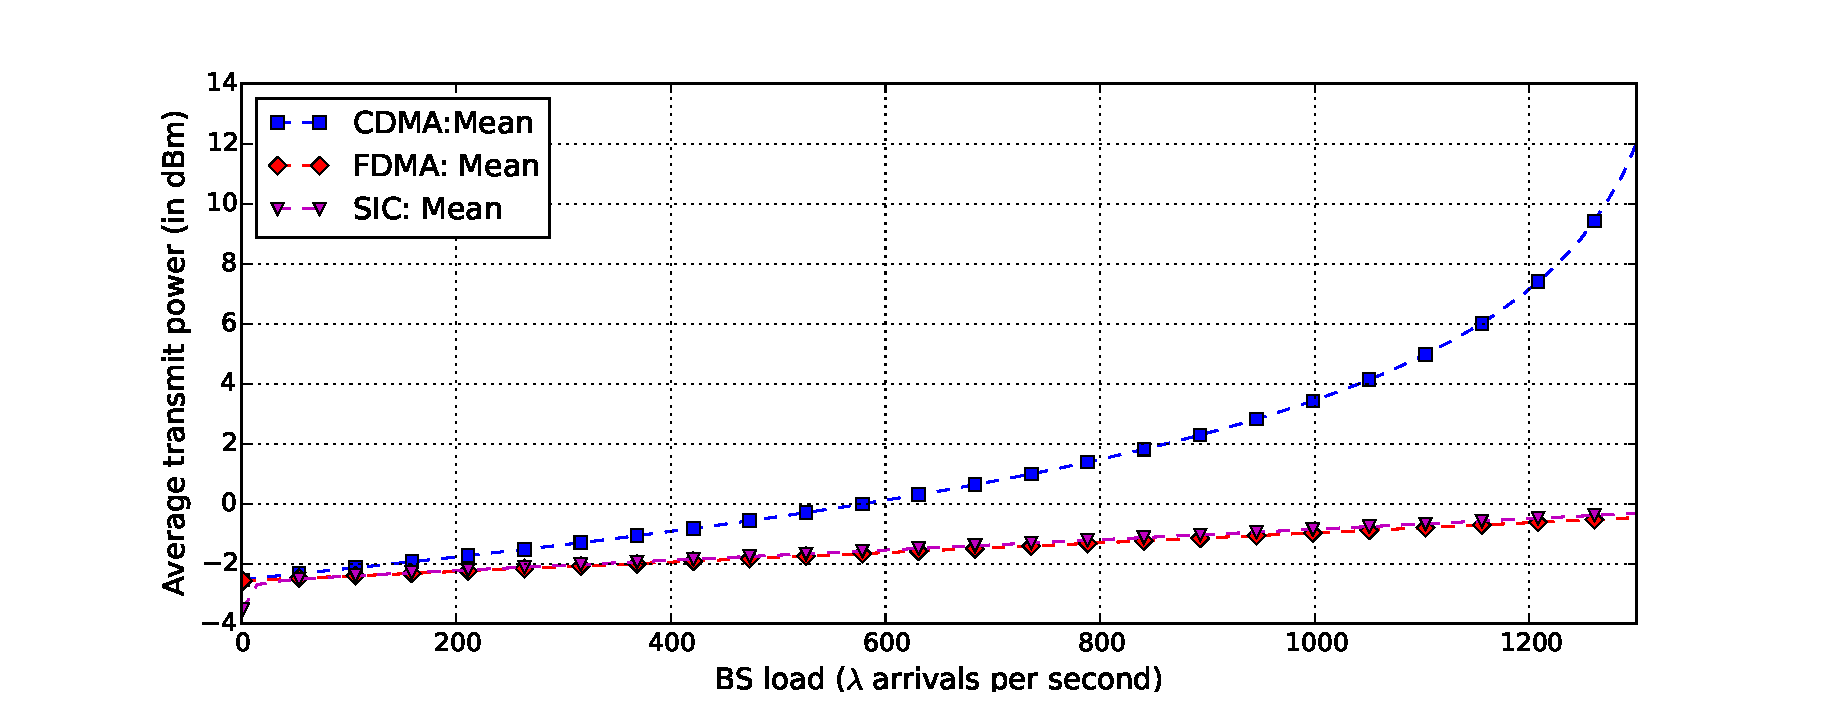
\includegraphics[width=0.5\textwidth, height=5cm]{Figures/Reproduction_Dhillon}
%	\caption{Comparison of power optimal solutions of SIC and FDMA with random access CDMA}
%	\label{fig:comparison-average-transmit-power}
%\end{figure}
\subsection{Impact of various packet length}
As discussed in previous section, the maximum supported base station load intensity is reduced when the maximum packet length increases.
The evolution of maximal packet length as to base station load intensity is illustrated in Fig.~\ref{fig:maximal-packet-length} according to inequality (\ref{ieq:packet-length-interval}). 
We evaluate the average transmit power between FDMA and CDMA under two different configurations where:\begin{inparaenum}[(i)]
	\item the packet length is constant and set as $1000$ bits;
	\item the packet length is variable varying from $1000$ bits to $3000$ bits.
\end{inparaenum}
As shown in Fig.~\ref{fig:maximal-packet-length}, to support a packet length up to $3000$ bits, the maximum base station supported load intensity is reduced to $400$ requests per second. This is the reason why the range of base station load is from $0$ to $400$ in the following figures. The evolution of power efficiency about base station load result is illustrated in Fig.~\ref{fig:Average-Transmit-Power-Variant-Target-SNR}. The curves with label reference case (CDMA or FDMA) respectively refer to the case where packet length payload $l$ is constant (namely $1000$ bits). Among all possible cases, both multiple access strategies achieve the best power efficient performance in reference case. The curve labeled \textit{\emph{CDMA:limit case}} illustrates the case where all MTC devices transfer packets with the length $3L$, which determines the upper bound limit for power consummation. All other possible cases should be between the CDMA limit case and reference case. For example, we assume packet length $l$ as a discrete random variable with distribution: $\mathbb{P}\{l=0.8L\} =0.2, \mathbb{P}\{l=1.0L\} =0.15, \mathbb{P}\{l=1.2L\} =0.15, \mathbb{P}\{l=1.6L\} =0.1, \mathbb{P}\{l=2L\} =0.1, \mathbb{P}\{l=2.5L\} =0.15, \mathbb{P}\{l=3L\} =0.15$, where $L=1000$ bits. The result associated to this configuration is shown by curve with label \textit{\emph{CDMA: general case}}.
From Fig.~\ref{fig:Average-Transmit-Power-Variant-Target-SNR}, we conclude that the coordinated FDMA strategy is more resistant to the variation of the packet length: its average transmit power increases slowly compared to that of CDMA. 

\begin{figure}[hb]
	\centering
	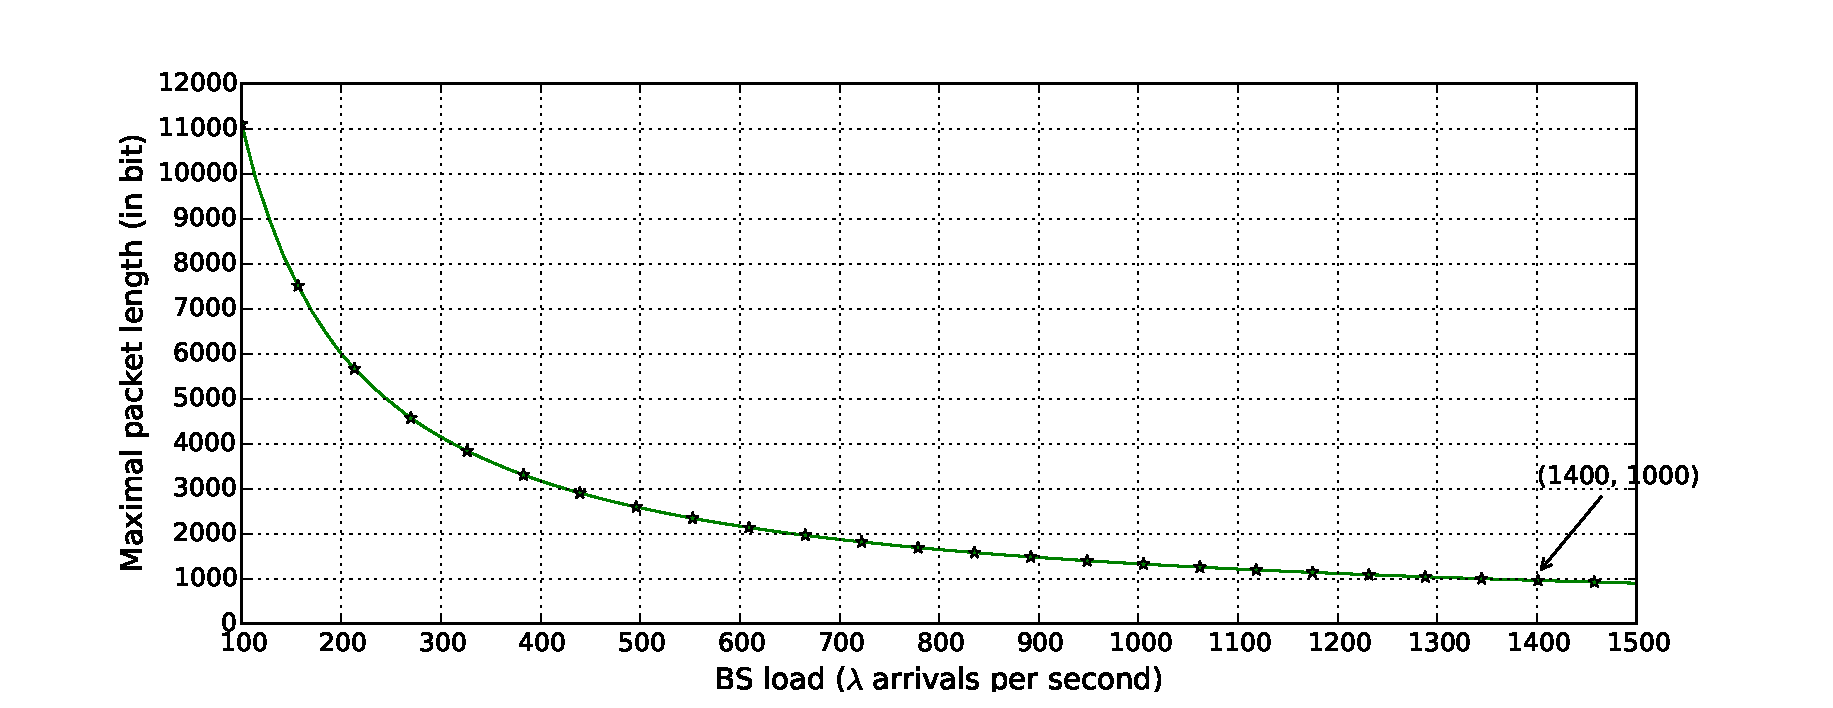
\includegraphics[width=0.5\textwidth, height=5cm]{Chapter3/Figures/Maximal-packet-length-evolution}
	\caption{Evolution of maximal packet length (in bit) with base station load intensity. For maximal packet length of 1000 bits, the maximum supported BS load is 1400.}
	\label{fig:maximal-packet-length}
\end{figure}
\begin{figure}[!tb]
	\centering
	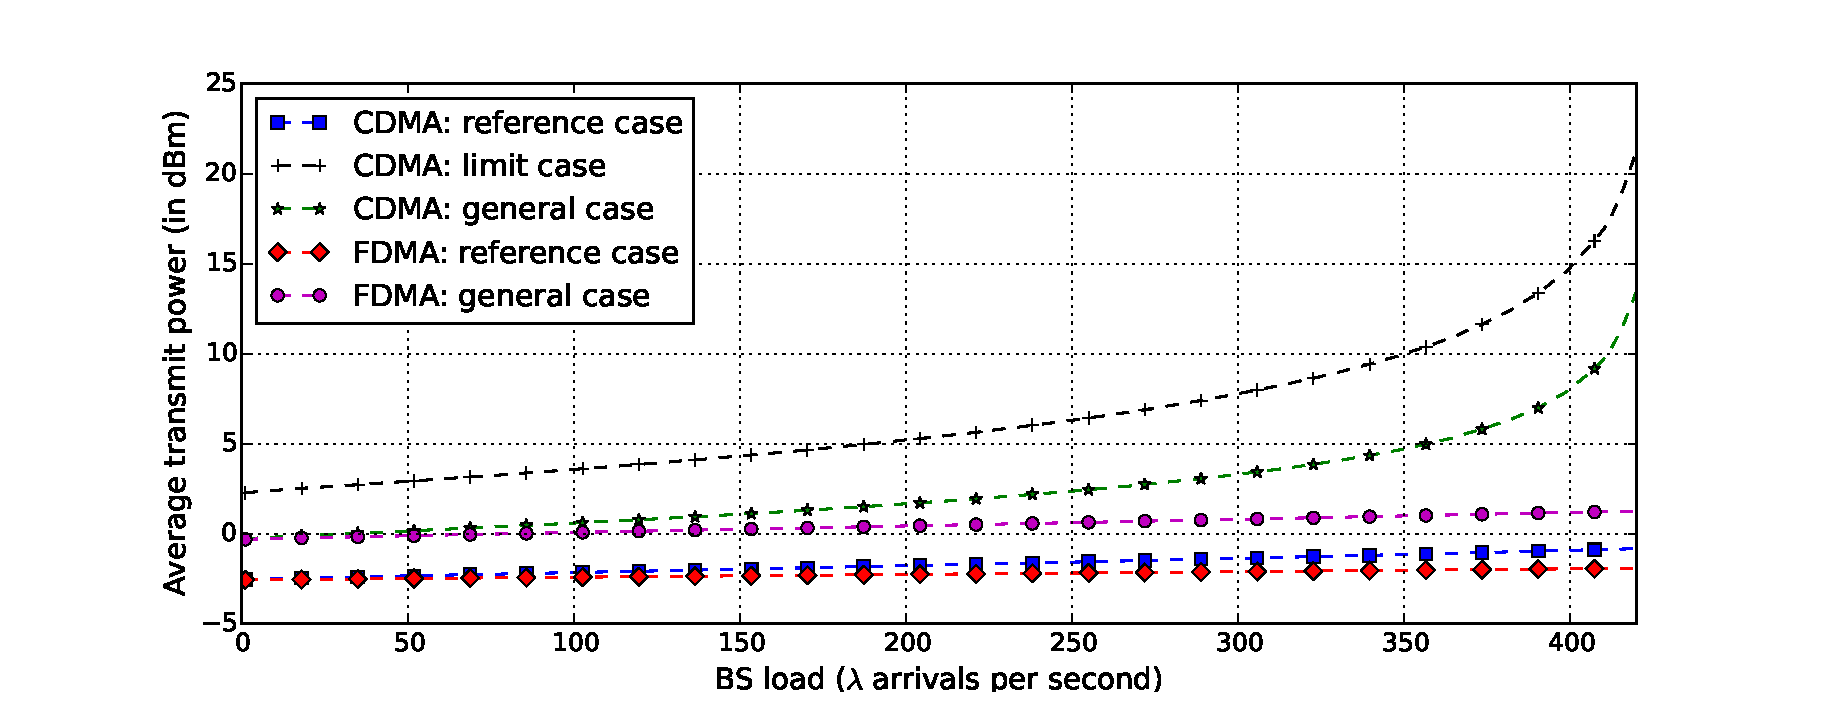
\includegraphics[width=0.5\textwidth, height=5cm]{Chapter3/Figures/Average-Transmit-Power-Variant-Target-SNR}
	\caption{Comparison of average transmit power with various packet length }
	\label{fig:Average-Transmit-Power-Variant-Target-SNR}
\end{figure}
\subsection{Imperfection of power control}
When evaluating the average transmit power under imperfect power control, we assume that the packet length $l$ is constant and set as $1000$ bits. Since it is complicated to obtain the closed-form expression for the term $C$ in formula (\ref{eq:imperfect-CDMA-transmit-power}), we take a statistical method to estimate the average transmit power for each given base station load intensity $\lambda$ and then draw the evolution curve of the average transmit power as a function of the base station load intensity. 
The numerical result where the variance of power control error $\sigma = 1$ is shown in Fig.~\ref{fig:imperfect-power-control-delta1}. The result of power control error variance $\sigma=1, 1.5$ is illustrated in Fig.~\ref{fig:imperfect-power-control-delta2}. 
The blue lines with full squares in both figures represent the case without power control error and thus serves as a reference case. The red scatter points represent the average transmit power with power control error variance $\sigma=1$, while the green scatter points are the case with power control error variance $\sigma=1.5$. From Fig.~\ref{fig:imperfect-power-control-delta1} and \ref{fig:imperfect-power-control-delta2}, the following conclusions are inferred \begin{inparaenum}[i)]
	\item the average transmit power increases when power control is imperfect;
	\item the power efficiency performance has the trend to degrade fast with a high power control error variance $\sigma$ when base station load increases.
\end{inparaenum}
\begin{figure}[!tb]
	\centering
	\includegraphics[width=0.5\textwidth, height=5cm]{Chapter3/Figures/Imperfect-power-control-CDMA-delta1-2015-1011}
	\caption{Comparison of average transmit power with power control error of variance $1$ }
	\label{fig:imperfect-power-control-delta1}
\end{figure}
\begin{figure}[!tb]
	\centering
	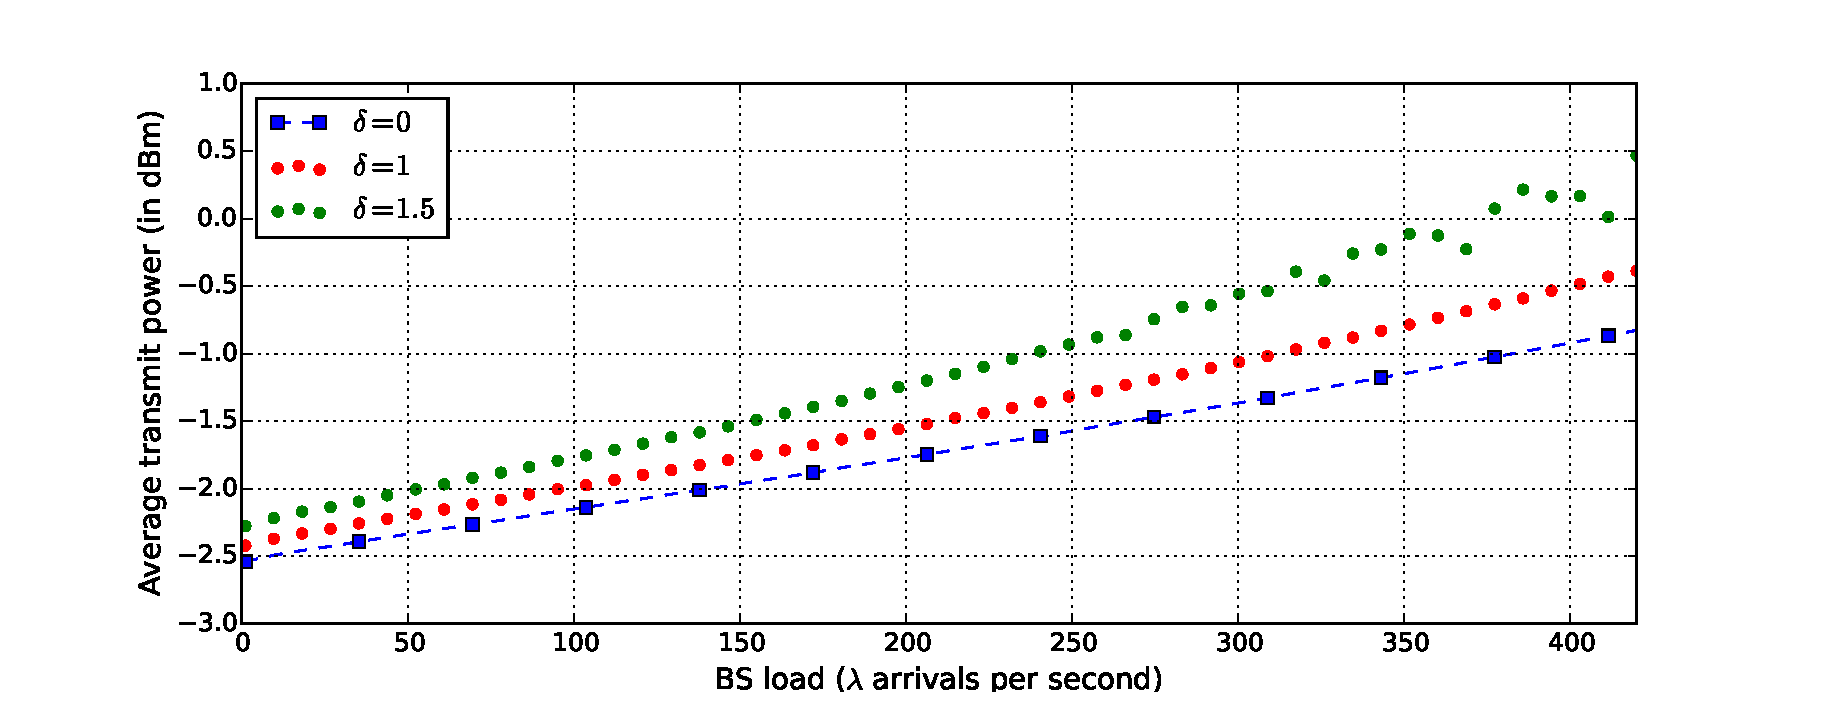
\includegraphics[width=0.5\textwidth,height=5cm]{Chapter3/Figures/Imperfect-power-control-CDMA-delta2-2015-1003}
	\caption{Comparison of average transmit power with power control error of variance $1$ and $1.5$ }
	\label{fig:imperfect-power-control-delta2}
\end{figure}
\section{Conclusion}
\label{sec:conclusion} 
%In this paper, we extend a previously proposed system model by taking into account the impact of variable packet length and the imperfect power control, and reevaluate the energy efficiency and system capacity for two typical multiple access strategies: uncoordinated CDMA and coordinated FDMA. The metric selected for measuring power efficiency is the average transmit power for devices situated in the circle area covered by a single cell. The energy efficiency is measured by the product of time and average transmit power. The system capacity is the maximum supported base station load intensity. The conclusions obtained from the comparison between uncoordinated CDMA and coordinated FDMA are: although uncoordinated CDMA exhibits features such as simplicity and no signaling overhead, it is not always a suitable multiple access for future M2M-included cellular networks. The arguments are following. First, compared with coordinated FDMA, the power efficiency of uncoordinated CDMA performance decreases significantly when BS load intensity increases, especially for the situation where there exist various packet lengths for M2M devices. Second, the power control is very important for the performance of uncoordinated CDMA, but with imperfect power control (which is inevitable in a piratical system), CDMA surely requires a higher level of transmit power, especially when power control error variance is large. Therefore, coordinated access strategy, especially FDMA, can often be a better choice for the future cellular network.
%
%New version:
In this paper, we extend a previously proposed system model by taking into account the impact of variable packet length and imperfect power control, and evaluate the energy efficiency and system capacity for two typical multiple access strategies: uncoordinated CDMA and coordinated FDMA. The metric selected for measuring power efficiency is the average transmit power for devices situated in the circle area covered by a single cell. The energy efficiency is measured by the product of time and average transmit power. The system capacity is the maximum supported base station load intensity. 
The conclusions obtained from the comparison between uncoordinated CDMA and coordinated FDMA are: 
coordinated access strategy, especially FDMA, can often be a better choice for the future cellular network.
Although with power control error, uncoordinated CDMA is a considerable multiple access schema for cellular M2M network dedicated for small data transmission due to its simplicity and no signaling overhead. However, the power efficiency performance of uncoordinated CDMA degrades significantly when BS load intensity increases. Furthermore, the system capacity, namely the maximum supported BS load intensity is rather limited when power control error is obvious.






